\chapterA{Hito 3 - Requisitos}

\section{Personas}

Tendremos dos personas, Marta (ver foto \ref{fig:fotoMarta}) e Isabel (ver foto \ref{fig:fotoIsaP}) \\

Para configurar estas personas, hemos utilizado un formato en el que vamos a dar en primer lugar la información general de la persona 
(edad, sexo, estudios y gustos). Posteriormente vamos a poner una foto de la persona (generada por una inteligencia artificial) y por último 
una descripción más elaborada de la persona, conteniendo la gran mayoría de los factoides e ideas expresadas en los esqueletos de las personas. 
Para poder destacar estas ideas, las hemos puesto en cursiva. \\

La estructura que van a tener las distintas personas va a seguir la siguiente configuración (ver figura \ref{fig:estructura-personas}) con los contenidos que hemos mecionado anteriormente.
\begin{figure}[h]
    \centering
    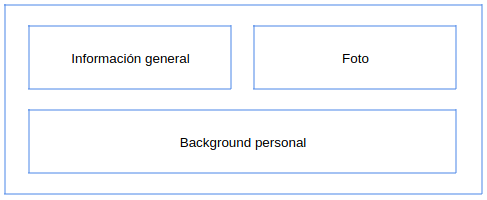
\includegraphics[width=0.5\textwidth]{Imagenes/Personas/Plantilla personas.png}
    \caption{Estructura de las personas}
    \label{fig:estructura-personas}
\end{figure}

\subsubsection{Marta González Torres}

\begin{minipage}{0.4\textwidth}
    \textbf{Información general} \\

    Edad: \textit{23 años} \\
    Sexo: Mujer \\
    Estudios: Ingeniería de Telecomunicaciones \\
    Gustos: Escuchar música e ir a conciertos cuando puede \\
\end{minipage}
\hfill
\begin{minipage}{0.4\textwidth}
    \centering
    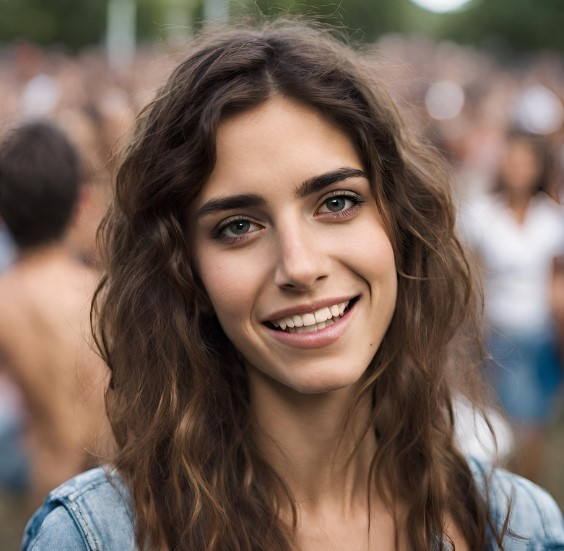
\includegraphics[width=0.5\textwidth]{Imagenes/Personas/Marta.jpg}
    \label{fig:fotoMarta}
    \captionof{figure}{Fotografía de Marta}
\end{minipage}

\textbf{Background personal} \\

Marta no puede salir de su casa sin los auriculares. Para ella la música es una gran parte
de su vida, y todas las mañanas, en la parada del bus, \textit{se prepara un playlist personalizada
en Spotify} para el itinerario hasta la Universidad. \textit{Vive en Fuenlabrada}, por lo que tiene
una ruta de una hora hasta que llega a Madrid, \textit{donde va a clase en la UCM}. \\ 

A Marta sobre todo le gusta la música italiana, ya que en el 2020 se fue de Erasmus a Turín y se
enamoró tanto de su cultura como de su música. Su cantante favorita es Francesca Michielin, así que
cuando hace gira intenta ir a algún concierto suyo en una \textit{ciudad italiana en la que no haya
estado}. De esta manera, puede conocer más la cultura italiana que tanto le gusta y sus diferenciados
a lo largo del país. \\

Se da la casualidad de que a su hermano Julián también le gusta mucho Francesca, así que en varias
ocasiones \textit{han ido ellos de viaje junto a sus padres} Carlos y Elena, los cuáles se van a
cenar juntos mientras sus hijos están en el concierto. \textit{Esto no lo hacen muy a menudo} debido
a que solo van cuando hay un concierto en alguna ciudad que les resulte interesante a toda la familia.
Normalmente se encarga ella de hacer la reserva tanto de los vuelos, \textit{para lo que usa
SkyScanner, como del alojamiento, utilizando AirBnB en este caso}. Esto se le hace a veces complicado
ya que quieren ir a varios sitios y tiene que cuadrar los horarios de todo. Por este motivo prefiere usar la 
aplicación web de las compañías, ya que así puede tener varias pestañas abiertas en las que visualiza toda
la información a la vez. \\

Con respecto al tema universitario, a Marta se le está haciendo cuesta arriba. Se metió inicialmente
en telecomunicaciones porque \textit{se le daban bien las matemáticas y la tecnología}, pero la
carrera no fue lo esperado. A pesar de las dificultades, la carrera le gusta y querría terminarla,
ya que este será en principio su último año. Pero estos problemas la agobian bastante, y para
distraerse le gusta mucho \textit{ir a festivales de música por España}. Suele ir todos los años
al festival Starlite, pues Pablo, el novio de su hermano y con el que mantiene muy buena relación,
es de Marbella, y se puede quedar algunos días en la playa aprovechando el viaje. Pero a pesar de
que no tiene que pagar gastos de alojamiento, el evento musical es bastante caro (ya que va varios
días), por lo que \textit{intenta ahorrar lo máximo posible en el viaje}. Para eso usa comparadores
de viaje como Omio, además de revisar las páginas de aerolíneas como \textit{RyanAir}, ya que a veces son
incluso más baratas que un vuelo o un tren.

\subsubsection{Isabel García Rodríguez}
\begin{minipage}{0.4\textwidth}
    \textbf{Información general} \\

    Edad: \textit{30 años} \\
    Sexo: Mujer \\
    Estudios: Psicología \\
    Gustos: Pintura y participar en grupos de apoyo para personas con discapacidad. \\
\end{minipage}
\hfill
\begin{minipage}{0.4\textwidth}
    \centering
    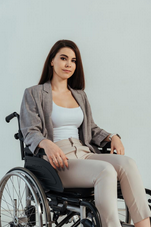
\includegraphics[width=0.5\textwidth]{Imagenes/Personas/Isabel.png}
    \label{fig:fotoIsaP}
    \captionof{figure}{Fotografía de Isabel}
\end{minipage}

\textbf{Background personal} \\

Isabel es una psicóloga comprometida con la mejora de la calidad de vida de las personas con discapacidad. \textit{Tiene una 
discapacidad física desde su nacimiento} que afecta su movilidad y requiere el uso de una silla de ruedas. Actualmente
\textit{vive en una pequeña urbanización a las afueras de Barcelona}. \\

Su familia vive en un pequeño pueblo de Huesca, por lo que \textit{siempre que puede se desplaza para verlos}. Muchas veces 
tiene el problema de la falta de autobuses que conectan con el pueblo, por lo que \textit{utiliza Omio, que realiza el trayecto
por ella, indicándole los transbordos que tiene que realizar y facilitándole la ayuda que necesita en todo momento}. \\

Ha asistido a varios cursos y conferencias relacionados con la psicología y la discapacidad, lo que la ha llevado a 
\textit{planear viajes a diferentes ciudades para participar en eventos}. Utiliza comparadores de viaje para encontrar opciones 
que se adapten a sus necesidades específicas, como hoteles con habitaciones adaptadas y \textit{vuelos con asistencia en el 
aeropuerto}. \textit{Algunos de los comparadores que usa no tienen opción de solicitar ayuda en caso de que tengas dudas, por lo que si
tiene algún problema no puede contactar con nadie}. Antes de realizar la reserva, ella sabe las distintas compañías y empresas que te lo suelen proporcionar. \\

Aparte de su trabajo, Isabel es una apasionada de la pintura y trata de visitar galerías y estudios de artistas en cada 
destino que visita. Isabel también es miembro activo de grupos de apoyo para personas con discapacidad en su ciudad. \textit{Allí 
es donde comparte experiencias y ofrece apoyo a otros miembros, por ejemplo a los jóvenes con discapacidad, para fomentar 
su independencia y autoestima}. Viaja a menudo con su mejor amiga, Carmen, quien la ha apoyado en su viaje de empoderamiento 
y ha aprendido mucho sobre la discapacidad en el proceso también.

\subsection{Tipos de personas}
\begin{itemize}
    \item \textbf{Persona Primaria} - \textit{Marta González Torres (Viajero que usa comparadores de viajes)} $\rightarrow$ Representa al tipo de usuario consumidor de comparadores de viajes. Se tratan de usuarios que utilizan activamente las funcionalidades de los comparadores con el objetivo de ahorrar lo máximo posible en los transportes para sus viajes.
    \item \textbf{Persona Secundaria} - \textit{Isabel García Rodríguez (Viajero con discapacidad)} $\rightarrow$ Representa al tipo de usuario consumidor o no consumidor de comparadores de viajes que tienen una necesidad añadida o distinta al resto de usuarios. 
    Generalmente usuarios que aparte de la interfaz ya creada necesitaran de una pequeña adaptación visual o sensorial para poder sacar el máximo provecho a la aplicación. En el caso de Isabel necesitaría un apoyo extra debido a su discapacidad que presenta, ya que sus viajes esterían mucho más condicionados que los de Marta.
\end{itemize}

\section{Problemas y visiones}

\begin{problema}

    Las personas que utilizan comparadores de viajes, en su gran mayoría, no tienen un gran poder adquisitivo: ``Suele ir todos los años al festival Starlite, pues Pablo, el novio de su hermano y con el que mantiene muy buena relación, es de Marbella, y se puede quedar algunos días en la playa aprovechando el viaje. Pero a pesar de que no tiene que pagar gastos de alojamiento, el evento musical es bastante caro (ya que va varios días), por lo que intenta ahorrar lo máximo posible en el viaje. Para eso usa comparadores de viaje como Omio.''

    {\centering\begin{vision}
    Nuestra aplicación ofrecerá los viajes más baratos al comienzo de la búsqueda cuando el usuario lo solicite dentro de unas fechas y una serie de filtros, además, podrá modificar filtrar la búsqueda ordenando las opciones como él prefiera.
    \end{vision}}
    \end{problema}
    
    \begin{problema}

    Las aplicaciones móviles son menos intuitivas que las webs: ``Para hacer este tipo de reservas prefiere utilizar aplicaciones web en vez de aplicaciones móviles ya que son más intuitivas.''

    {\centering\begin{vision}
    Nuestra app va a ofrecer la información justa y necesaria, sacaremos una versión ``Alpha'' para poder aprender de ella y mejorarla a través del uso.
    \end{vision}}
    \end{problema}
    
    \begin{problema}

    Los sitios a los que viajar tienen que tener un amplio abanico de posibilidades culturales y/o recreativas: ``Se da la casualidad de que a su hermano Julián también le gusta mucho Francesca, así que en varias ocasiones han ido ellos de viaje junto a sus padres Carlos y Elena, los cuales se van a cenar juntos mientras sus hijos están en el concierto. Esto no lo hacen muy a menudo debido a que solo van cuando hay un concierto en alguna ciudad que les resulte interesante a toda la familia.''

    {\centering\begin{vision}
    Nuestra aplicación ofrecerá unas recomendaciones en la página de inicio acorde a los gustos y preferencias del usuario, las cuales serán obtenidas a través de cookies.
    \end{vision}}
    \end{problema}
    
    \begin{problema}

    Numerosas aplicaciones web o móviles no están adaptadas a las diferentes discapacidades que puedan poseer los usuarios: ``Tiene una discapacidad física desde su nacimiento.''

    {\centering\begin{vision}
    Nuestra aplicación contará con el Nivel Triple-A de Conformidad con las Directrices de Accesibilidad para el Contenido Web 1.0 (WCAG 1.0) para ser accesible para todo tipo de usuarios.
    \end{vision}}
    \end{problema}
    
    \begin{problema}

    No conocer de antemano toda la información y/o ventajas de las que se disponga: ``Algunos de los comparadores que usa no tienen opción de solicitar ayuda en caso de que tengas dudas, por lo que si tiene algún problema no puede contactar con nadie. Antes de realizar la reserva, ella sabe las distintas compañías y empresas que te lo suelen proporcionar.''

    {\centering\begin{vision}
    Nuestra aplicación contará con un apartado de ventajas/descuentos con toda la información detallada así como con un apartado en el que estarán especificados los servicios que ofrecemos. También contaremos con un chat en directo, una página de preguntas frecuentes y un formulario de contacto para poder hacer frente a cualquier duda que pueda tener el usuario.
    \end{vision}}
    \end{problema}
    
    \begin{problema}

    Las personas con discapacidad física muchas veces deben hacer un esfuerzo extra a la hora de saber si pueden reservar un viaje en algún transporte ya que no viene de forma clara que exista una adaptabilidad para estas personas: ``Muchas veces ha tenido que contactar directamente con el aeropuerto o estación de tren para conocer los servicios que ofrecen. Le gustaría que los comparadores tuvieran más información al respecto.''
    
    {\centering\begin{vision}
    Nuestra aplicación contará con toda la información sobre las diferentes discapacidades y cómo poder ayudar a los distintos usuarios así como nuestros trabajadores poseerán la información necesaria para poder contactar con las diferentes empresas de transporte y poder mediar entre el usuario y la empresa para poder viajar cómodo y seguro sin preocupaciones.
    \end{vision}}
    \end{problema}
    
